\section{Tree}
\label{sec:Tree}
%%%%%%%%%%%%%%%%%%%%%%%%%%%%%%%%%%%%%%%%%%%%%%%%%%%%%%%%
\begin{figure}[h!]
\begin{center}
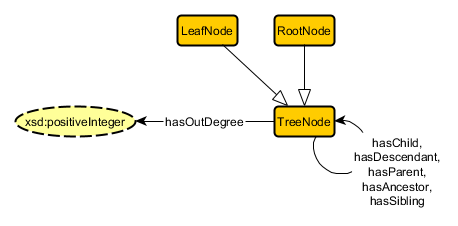
\includegraphics[width=.8\textwidth]{figures/tree}
\end{center}
\caption{Schema Diagram for the Tree Pattern. The visual notation is explained in Chapter \ref{chap:prelims}.}
\label{fig:Tree}
\end{figure}
\subsection{Summary}
\label{sum:Tree}
%%%%%%%%%%%%%%%%%%%%%%%%%%%%
The \textsf{Tree} pattern allows a developer to organize data into a tree data structure. An ontological tree, however, is subtly different from those that occur in other parts of computer science; these trees should be viewed as static---something to be queried, not manipulated. For example, a motivating use case is the organization of organisms into a phylogenetic tree. Such examples and more information may be found in \cite{tree}, from where this pattern is adapted.

%%%%%%%%%%%%%%%%%%%%%%%%%%%%%%%%%%%%%%%%%%%%%%%%%%%%%%%%
\subsection{Axiomatization}
\label{axs:Tree}
%%%%%%%%%%%%%%%%%%%%%%%%%%%%
\begin{align}
\textsf{LeafNode} &\sqsubseteq \textsf{TreeNode} \\ 
\textsf{RootNode} &\sqsubseteq \textsf{TreeNode} \\ 
\textsf{TreeNode} &\sqsubseteq \forall \textsf{hasOutDegree.xsd:positiveInteger} \\ 
\textsf{TreeNode} &\sqsubseteq \mathord{=1}\textsf{hasOutDegree.xsd:positiveInteger} \\ 
\textsf{LeafNode} &\equiv \textsf{TreeNode} \sqcap \forall \textsf{hasOutDegree.} \{ 0 \textsf{\^{}\^{}xsd:positiveInteger}\} \\ 
\textsf{TreeNode} \sqcap \lnot \textsf{LeafNode} &\equiv \textsf{TreeNode} \sqcap \forall \textsf{hasOutDegree.}\{ x\textsf{\^{}\^{}xsd:positiveInteger} | 1 \leq x\} \\
\textsf{hasChild} &\equiv \textsf{hasParent}^- \\ 
\textsf{hasDescendant} &\equiv \textsf{hasAncestor}^- \\ 
\textsf{hasChild} &\sqsubseteq \textsf{hasDescendant} \\ 
\textsf{hasDescendant} \circ \textsf{hasDescendant} &\sqsubseteq \textsf{hasDescendant} \\ 
\textsf{TreeNode} &\sqsubseteq \forall \textsf{hasChild.TreeNode} \\ 
\textsf{TreeNode} \sqcap \lnot \textsf{LeafNode} &\equiv \textsf{TreeNode} \sqcap \exists \textsf{hasChild.TreeNode} \\ 
\textsf{TreeNode} &\sqsubseteq \forall \textsf{hasDescendant.TreeNode} \\ 
\textsf{TreeNode} &\sqsubseteq \forall \textsf{hasParent.TreeNode} \\ 
\textsf{TreeNode} &\sqsubseteq \forall \textsf{hasSibling.TreeNode} \\ 
\textsf{TreeNode} \sqcap \lnot \textsf{RootNode} &\equiv \textsf{TreeNode} \sqcap \mathord{=1}\textsf{hasParent.}\top \\ 
\textsf{TreeNode} &\sqsubseteq \forall \textsf{hasAncestor.TreeNode} \\ 
\textsf{RootNode} &\equiv \textsf{TreeNode} \sqcap \lnot\exists \textsf{hasParent.}\top \\ 
\textsf{LeafNode} &\equiv \textsf{TreeNode} \sqcap \lnot\exists \textsf{hasChild.}\top \\ 
\text{Irreflexive}&(\textsf{hasChild}) \\ 
\text{Irreflexive}&(\textsf{hasParent}) \\ 
\text{Irreflexive}&(\textsf{hasDescendant}) \\ 
\text{Irreflexive}&(\textsf{hasAncestor}) \\ 
\textsf{hasSibling} &\equiv \textsf{hasSibling}^- \\ 
\text{Irreflexive}&(\textsf{hasSibling})
\end{align}

%%%%%%%%%%%%%%%%%%%%%%%%%%%%%%%%%%%%%%%%%%%%%%%%%%%%%%%%
\subsection{Explanations}
\label{exp:Tree}
%%%%%%%%%%%%%%%%%%%%%%%%%%%%
\begin{enumerate}
\item Subclass: every \textsf{LeafNode} is a \textsf{TreeNode}.
\item Subclass: the \textsf{RootNode} is a \textsf{TreeNode}.
\item Scoped Range: the range of \textsf{hasOutDegree}, scoped by \textsf{TreeNode}, is \textsf{xsd:positiveInteger}.
\item Existential: a \textsf{TreeNode} has exactly one \textsf{hasOutDegree}.
\item A \textsf{LeafNode} is a \textsf{TreeNode} that has an out degree of 0.
\item A \textsf{TreeNode} that is not a \textsf{LeafNode} has at least out degree of 1.
\item Inverse Alias
\item Inverse Alias
\item Subproperty: \textsf{hasChild} is subproperty of \textsf{hasDescendant}.
\item Role Chain: \textsf{hasDescendant} is transitive.
\item Scoped Range: the range of \textsf{hasChild}, scoped by \textsf{TreeNode}, is \textsf{TreeNode}.
\item A \textsf{TreeNode} that is not a \textsf{LeafNode} has a child that is a \textsf{TreeNode}.
\item Scoped Range: the range of \textsf{hasDescendant}, scoped by \textsf{TreeNode}, is \textsf{TreeNode}.
\item Scoped Range: the range of \textsf{hasParent}, scoped by \textsf{TreeNode}, is \textsf{TreeNode}.
\item Scoped Range: the range of \textsf{hasSibling}, scoped by \textsf{TreeNode}, is \textsf{TreeNode}.
\item A \textsf{TreeNode} that is not the \textsf{RootNode} has a \textsf{TreeNode} that is its parent.
\item Scoped Range: the range of \textsf{hasAncestor}, scoped by \textsf{TreeNode}, is \textsf{TreeNode}.
\item \textsf{RootNode} does not have a \textsf{TreeNode} that is its parent.
\item \textsf{LeafNodes} do not have \textsf{TreeNodes} that are its children.
\item Irreflexivity
\item Irreflexivity
\item Irreflexivity
\item Irreflexivity
\item Inverse Alias
\item Irreflexivity
\end{enumerate}

%%%%%%%%%%%%%%%%%%%%%%%%%%%%%%%%%%%%%%%%%%%%%%%%%%%%%%%%
\subsection{Competency Questions}
\label{cqs:Tree}
%%%%%%%%%%%%%%%%%%%%%%%%%%%%
We remark that these competency questions are as general as the pattern. See \cite{tree} for more information.
\begin{enumerate}[CQ1.]
\item Determine the root.
\item Determine all ancestors of a given node.
\item Determine all leaves.
\item Determine all descendants of a given node.
\item Determine all descendants of a given node which are leaves.
\item Given two nodes, determine whether one is a descendant of the other.
\item given two nodes, determine all common ancestors.
\item Given two nodes, determine the latest common ancestor.
\item Given two nodes $x$ and $y$, determine the earliest ancestor of $x$ which not an ancestor of $y$.
\end{enumerate}

\newpage
%%%%%%%%%%%%%%%%%%%%%%%%%%%%%%%%%%%%%%%%%%%%%%%%%%%%%%%%
% End Section
%%%%%%%%%%%%%%%%%%%%%%%%%%%%%%%%%%%%%%%%%%%%%%%%%%%%%%%%
%%%%%%%%%%%%%%%%%%%%%%%%%%%%%%%%%%%%%%%%%%%%%%%%%%%%%%%%